\section{System architecture}\label{sec:system-architecture}

The Papaya software consists of three essential parts.
Those are:
\begin{itemize}
    \item Papaya Keycloak --- a Keycloak authentication server, it provides
    authentication, authorization, and user management services;
    \item Papaya Backend --- a web application which provides the
    business logic and is the core part of the project;
    \item Papaya Frontend --- a web application responsible for serving web
    pages, it provides GUI for Papaya Backend.
\end{itemize}
The figure~\ref{fig:architecture-diagram} shows dependencies between those
services.

\begin{figure}[!h]
    \centering
    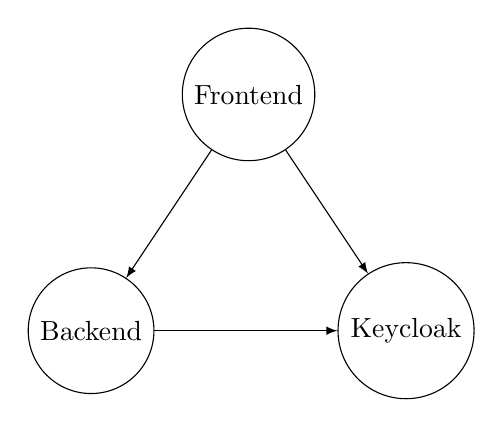
\begin{tikzpicture}
    \node[draw, circle] (f) at (2, 3) {Frontend};
    \node[draw, circle] (b) at (0, 0) {Backend};
    \node[draw, circle] (k) at (4, 0) {Keycloak};
    \draw[->, >=latex] (f) -- (k);
    \draw[->, >=latex] (f) -- (b);
    \draw[->, >=latex] (b) -- (k);
\end{tikzpicture}

    \caption{Architecture diagram}
    \label{fig:architecture-diagram}
\end{figure}

Keycloak is an auth server used by Papaya to manage users and
provide secure authentication.
There are several reasons to use it, such as:
\begin{itemize}
    \setlength\itemsep{0.1em}
    \item it natively supports SSL protection,
    \item it allows user registration,
    \item it provides single sign-on/sign-off across all
    applications belonging to the same realm,
    \item 2-factor authentication,
    \item LDAP synchronization.
\end{itemize}
